
\documentclass[12pt]{article}
%\setlength{\oddsidemargin}{0in}
%\setlength{\evensidemargin}{0in}
%\setlength{\textwidth}{6.5in}
%\setlength{\parindent}{0in}
%\setlength{\parskip}{\baselineskip}
\thispagestyle{empty}
\usepackage{fullpage}
\usepackage{amsmath,amsthm,amsfonts}
\usepackage{graphicx, graphics}
\usepackage[usenames,dvipsnames]{color}

\definecolor{darkyellow}{rgb}{.929412,.8314,0}
\definecolor{brightgreen}{rgb}{.439,.824,.0863}


\newtheorem*{thm}{Theorem}

\begin{document}

%=======================================================
\begin{center}
{\large \bf Comments for Lecture 8}\\
\bf{2.5.2010}
\end{center}


\begin{center}
{\bf Matrix Multiplication}.  
\end{center}

Suppose $A$ is a $p\times m$ matrix and $B$ is a $m\times n$ matrix.  Then we can define the product $C=AB$ as the $p\times n$ matrix such that

\[
c_{ij} = a_{i1}b_{1j} + a_{i2}b_{2j} + \ldots + a_{im}b_{mj}
 \]

\noindent {\bf NOTE:} there was a typo in the text on page 55 for formula (2.2). The sum definitely goes up to $m$ and NOT $n$.  So the sum should read:
\[c_{ij}=\sum_{k=1}^m a_{ik} b_{kj} \] (as we have above)

\noindent  Also there is another minor typo in (2.1), it should read: ${\bf r}_i^{'}=a_{i1}{\bf r}_1+a_{i2}{\bf r}_2+\ldots+a_{im}{\bf r}_m$, where the prime was missing in the text).

The books has a nice way to visualize matrix multiplication (similar to the image below).  Suppose for example $A$ is a $3 \times 2$ matrix and $B$ is a $2 \times 3$ matrix.  The resulting product $AB$ will be a $3 \times 3$ matrix such that 

\[ c_{ij} = a_{i1}b_{1j} + a_{i2}b_{2j} \]

\noindent as we have seen above.  Visually\footnote{ \texttt{http://en.wikipedia.org/wiki/File:Matrix\textunderscore multiplication\textunderscore diagram\textunderscore 2.svg} }:
\begin{figure}[h!]
  \centering
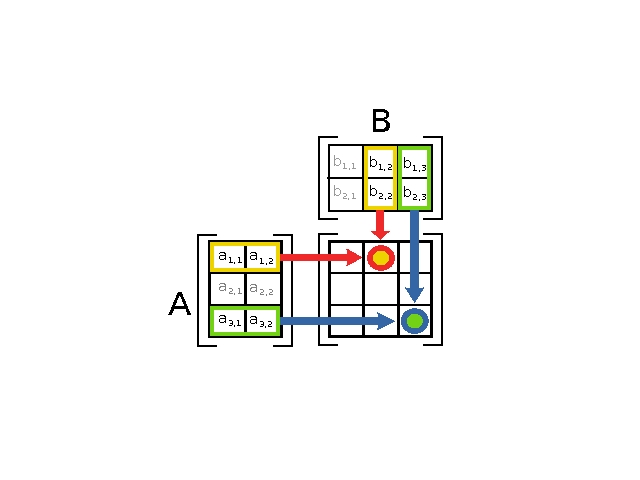
\includegraphics[height=70mm]{mult.jpg}
\end{figure}

So for example the entry \colorbox{darkyellow}{$c_{12}$} = $a_{11}b_{12}+a_{12}b_{22}$ and the entry \colorbox{brightgreen}{$c_{33}$} = $a_{31}b_{13}+a_{32}b_{23}$.

\noindent Please read section {\bf 2.2.2 Getting used to the formula}.  Understanding this product is absolutely necessary! \\

\noindent We really need to practice so I would recommend working through every problem from ``{\bf Exercises (15)}" on page 60-62.  Most of these will be a part of homework 3.

%=======================================================

\end{document}
